
To evaluate the risk of disclosure, we use a measure proposed for evaluating the disclosure risks of the SynLBD \citep{KinneyEtAl2011}: For each industry, we estimate the probability that the synthetic birth year equals the true birth year, conditional on the synthetic birth year. Tables~\ref{tab:Can:ProbabilityPrivate} and \ref{tab:GLBD:Probability} show that these probabilities are quite low except for the first year. Entry rates in the first year are much larger than in any other year due to censoring. It is therefore to be expected that there is a high probability that the entry year of the synthetic record matches that of the original record if the synthetic entry year is the first year observed in the data. For the German data, we see another spike in the match rates for the years 1991 and 1992. These are the years in which data from Eastern Germany were added to the database successively. Thus, the increase in match rates can be attributed to increased entry rates in those two years. 
The probability for the first year is higher because of censoring and lack of previous information.

\begin{table}[H]
\centering\footnotesize
\caption{Observed entity births given synthetic births for LEAP.} \label{tab:Can:ProbabilityPrivate} \medskip
\renewcommand{\arraystretch}{1}
\begin{tabular}{c c| c c c}
\toprule
\multicolumn{2}{c|}{\textbf{First (Birth) Year}} &  \multicolumn{3}{c}{\textbf{\% of Births over NAICS}}\\
\textbf{Synthetic}&\textbf{Actual}&\textbf{Minimum}&\textbf{Mean}&\textbf{Maximum}\\
\midrule
1991&1991&0.00&27.69&83.02\\
1992&1992&0.00&3.37&11.11\\
1993&1993&0.00&3.79&33.33\\
1994&1994&0.00&3.73&33.33\\
1995&1995&0.00&3.86&20.00\\
1996&1996&0.00&4.25&33.33\\
1997&1997&0.00&4.10&16.94\\
1998&1998&0.00&4.41&25.00\\
1999&1999&0.00&4.23&33.33\\
2000&2000&0.00&3.41&25.00\\
2001&2001&0.00&2.73&22.22\\
2002&2002&0.00&2.65&25.00\\
2003&2003&0.00&2.22&10.00\\
2004&2004&0.00&2.60&17.86\\
2005&2005&0.00&2.71&20.00\\
2006&2006&0.00&2.83&50.00\\
2007&2007&0.00&2.90&33.33\\
2008&2008&0.00&2.38&20.00\\
2009&2009&0.00&2.47&50.00\\
2010&2010&0.00&2.12&33.33\\
2011&2011&0.00&2.65&50.00\\
2012&2012&0.00&2.41&20.00\\
2013&2013&0.00&2.48&25.00\\
2014&2014&0.00&2.23&20.00\\
2015&2015&0.00&2.15&33.33\\

\bottomrule
\end{tabular} 
\\
\justify
%Note:
\end{table}

%\begin{table}[H]
%\centering\footnotesize
%\caption{Observed entity births given synthetic births %(manufacturing)} \label{tab:Can:ProbabilityManufacturing} \medskip
%\renewcommand{\arraystretch}{1}
%\begin{tabular}{c c| c c c}
%\toprule
%\multicolumn{2}{c|}{\textbf{Birth Year}} &  \multicolumn{3}{c}{\textbf{\% of Births over NAICS}}\\
%\textbf{Synthetic}&\textbf{Actual}&\textbf{Minimum}&\textbf{Mean}&\textbf{Maximum}\\
%\midrule
%1991&1991&4.76&31.64&52.03\\
1992&1992&0.00&3.32&10.53\\
1993&1993&0.00&3.97&33.33\\
1994&1994&0.00&4.21&33.33\\
1995&1995&0.00&4.41&20.00\\
1996&1996&0.00&5.36&33.33\\
1997&1997&0.00&4.09&16.94\\
1998&1998&0.00&5.46&25.00\\
1999&1999&0.00&5.27&33.33\\
2000&2000&0.00&3.39&25.00\\
2001&2001&0.00&2.19&10.00\\
2002&2002&0.00&2.45&25.00\\
2003&2003&0.00&1.71&10.00\\
2004&2004&0.00&2.07&17.86\\
2005&2005&0.00&1.92&16.67\\
2006&2006&0.00&2.49&50.00\\
2007&2007&0.00&1.74&14.29\\
2008&2008&0.00&1.60&20.00\\
2009&2009&0.00&1.60&20.00\\
2010&2010&0.00&1.34&33.33\\
2011&2011&0.00&2.43&50.00\\
2012&2012&0.00&1.93&20.00\\
2013&2013&0.00&1.61&20.00\\
2014&2014&0.00&1.71&14.29\\
2015&2015&0.00&1.41&14.29\\

%\bottomrule
%\end{tabular} 
%\\
%\justify
%Note:
%\end{table}

\begin{table}[H]\label{tab:GLBD:Probability}
\centering\footnotesize
\caption{Observed entity births given synthetic births (GLBD)} \label{ProbabilityManufacturing} \medskip
\renewcommand{\arraystretch}{1}
\begin{tabular}{c c| c c c}
\toprule
\multicolumn{2}{c|}{\textbf{Birth Year}} &  \multicolumn{3}{c}{\textbf{\% of Births over NAICS}}\\
\textbf{Synthetic}&\textbf{Actual}&\textbf{Minimum}&\textbf{Mean}&\textbf{Maximum}\\
\midrule
1976&1976&1.55&1.62&1.68\\
1977&1977&1.35&1.55&1.75\\
1978&1978&0.97&1.50&2.02\\
1979&1979&1.99&2.05&2.11\\
1980&1980&1.15&1.61&2.07\\
1981&1981&0.76&1.28&1.80\\
1982&1982&1.29&1.39&1.48\\
1983&1983&1.54&1.57&1.61\\
1984&1984&0.99&1.03&1.07\\
1985&1985&0.83&1.56&2.28\\
1986&1986&1.36&1.79&2.21\\
1987&1987&1.99&2.00&2.02\\
1988&1988&1.18&1.49&1.81\\
1989&1989&1.65&1.84&2.03\\
1990&1990&2.44&2.79&3.14\\
1991&1991&7.59&9.17&10.75\\
1992&1992&5.19&8.81&12.42\\
1993&1993&3.20&3.40&3.60\\
1994&1994&3.50&3.93&4.35\\
1995&1995&2.86&3.26&3.65\\
1996&1996&1.89&2.62&3.35\\
1997&1997&3.46&3.96&4.45\\
1998&1998&3.58&3.68&3.78\\
1999&1999&5.56&5.78&6.00\\
2000&2000&3.19&3.64&4.10\\
2001&2001&3.26&3.59&3.93\\
2002&2002&2.04&3.00&3.97\\
2003&2003&2.13&3.17&4.20\\
2004&2004&2.57&3.24&3.91\\
2005&2005&1.66&2.54&3.41\\
2006&2006&2.15&3.06&3.97\\
2007&2007&2.17&2.90&3.62\\
2008&2008&2.37&2.42&2.47\\
2009&2009&0.00&0.00&0.00\\
2010&2010&0.00&0.00&0.00\\

\bottomrule
\end{tabular} 
\\
\justify
%Note:
\end{table}

%\begin{figure} [H]
%\centering
%\caption{The difference between first and last year given synthetic first year} \label{SyntheticFirstYear}
%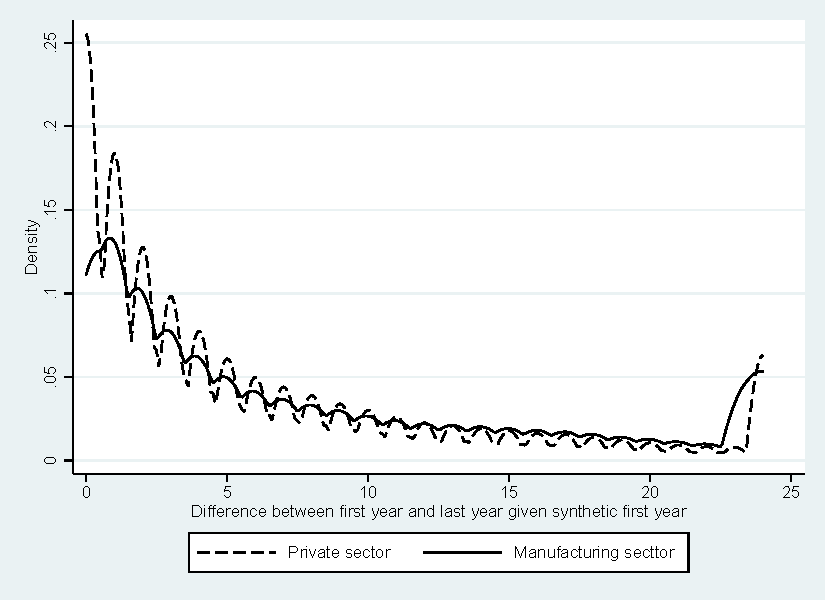
\includegraphics[height=2.8in, width=.7\linewidth]{graphs/The_difference_between_first_and_last_year_given_synthetic_first_year_bw.pdf} 
%\begin{minipage}{0.85\textwidth}
%{\footnotesize Note:  \par}
%\end{minipage}
%\end{figure}
